\section{Kết quả và diễn giải}

\subsection{Kiểm tra dữ liệu}
Validation đạt cho observations train, nhãn RUL train và observations test. Tập
train có 20.631 dòng, tập test có 13.096 dòng; mỗi tập gồm 100 engine. Một trăm
test labels hợp lệ về cấu trúc nhưng được giữ tách khỏi EDA và suy luận trên
train. Các kiểm tra schema, khóa duy nhất, kiểu số hữu hạn và cycle liên tục đều
đạt.

\subsection{ETL Silver/Gold và benchmark}
Pipeline Pandas và PySpark đọc dữ liệu sau khi kiểm tra data contract. Silver gồm
33.727 observations train/test và 20.631 train targets. Gold gồm 200 dòng engine
summary trong Parquet và bảng truy vấn tương ứng trong SQLite. Các bảng được đọc
lại sau khi ghi.

\begin{table}[H]
\centering
\caption[Benchmark Pandas tạo engine summary]{Benchmark tạo engine summary trên
observations nhân bản trong bộ nhớ; dữ liệu nhân bản không dùng để huấn luyện.}
\label{tab:etl-benchmark}
\begin{tabular}{rrrrr}
\toprule Scale & Input rows & Engine rows & Cold (s) & Warm (s)\\\midrule
1$\times$ & 33.727 & 200 & 0,0195 & 0,0196\\
10$\times$ & 337.270 & 2.000 & 0,1589 & 0,1474\\
100$\times$ & 3.372.700 & 20.000 & 1,6752 & 1,6732\\
\bottomrule
\end{tabular}
\end{table}

Benchmark đo chi phí của phép tổng hợp cục bộ, không phải bằng chứng về xử lý
phân tán. Pandas và PySpark khớp schema, khóa, số dòng và giá trị số cho ba bảng
Silver/Gold; sai khác tuyệt đối lớn nhất đều bằng 0,0.

\subsection{Rolling features}
Rolling features dài 30 cycles gồm 17.731 train windows và 10.196 test windows,
tổng cộng 27.927 dòng. Mỗi dòng có khóa \texttt{(split, engine\_id, cycle)} và
126 feature columns cho 21 sensor, gồm \texttt{last}, \texttt{mean}, sample
\texttt{std}, \texttt{min}, \texttt{max} và \texttt{slope}. Test labels không
được ghép trong bước này.

\begin{table}[H]
\centering
\caption[Rolling features theo split]{Số rolling windows theo split.}
\label{tab:rolling-features}
\begin{tabular}{lrr}
\toprule Split & Engines & Rolling windows\\\midrule
Train & 100 & 17.731\\
Test & 100 & 10.196\\
Tổng & 200 & 27.927\\\bottomrule
\end{tabular}
\end{table}

Validator kiểm tra schema, khóa duy nhất, thứ tự canonical, số hữu hạn và đủ
trailing window trong từng engine. Tests tính tay xác nhận sample standard
deviation, slope, không dùng tương lai và không nối hai engine.

\subsection{Tuổi thọ động cơ trên train}
\begin{table}[H]
\centering
\caption[Thống kê tuổi thọ của 100 động cơ train]{Thống kê tuổi thọ, đơn vị
cycle.}
\label{tab:lifetime}
\begin{tabular}{lr@{\qquad}lr}
\toprule Thống kê & Giá trị & Thống kê & Giá trị\\\midrule
Trung bình & 206,31 & Độ lệch chuẩn mẫu & 46,34\\
Nhỏ nhất & 128 & Lớn nhất & 362\\
Tứ phân vị 25\% & 177 & Trung vị & 199\\
Tứ phân vị 75\% & 229,25 & Số động cơ & 100\\\bottomrule
\end{tabular}
\end{table}

\begin{figure}[H]
\centering
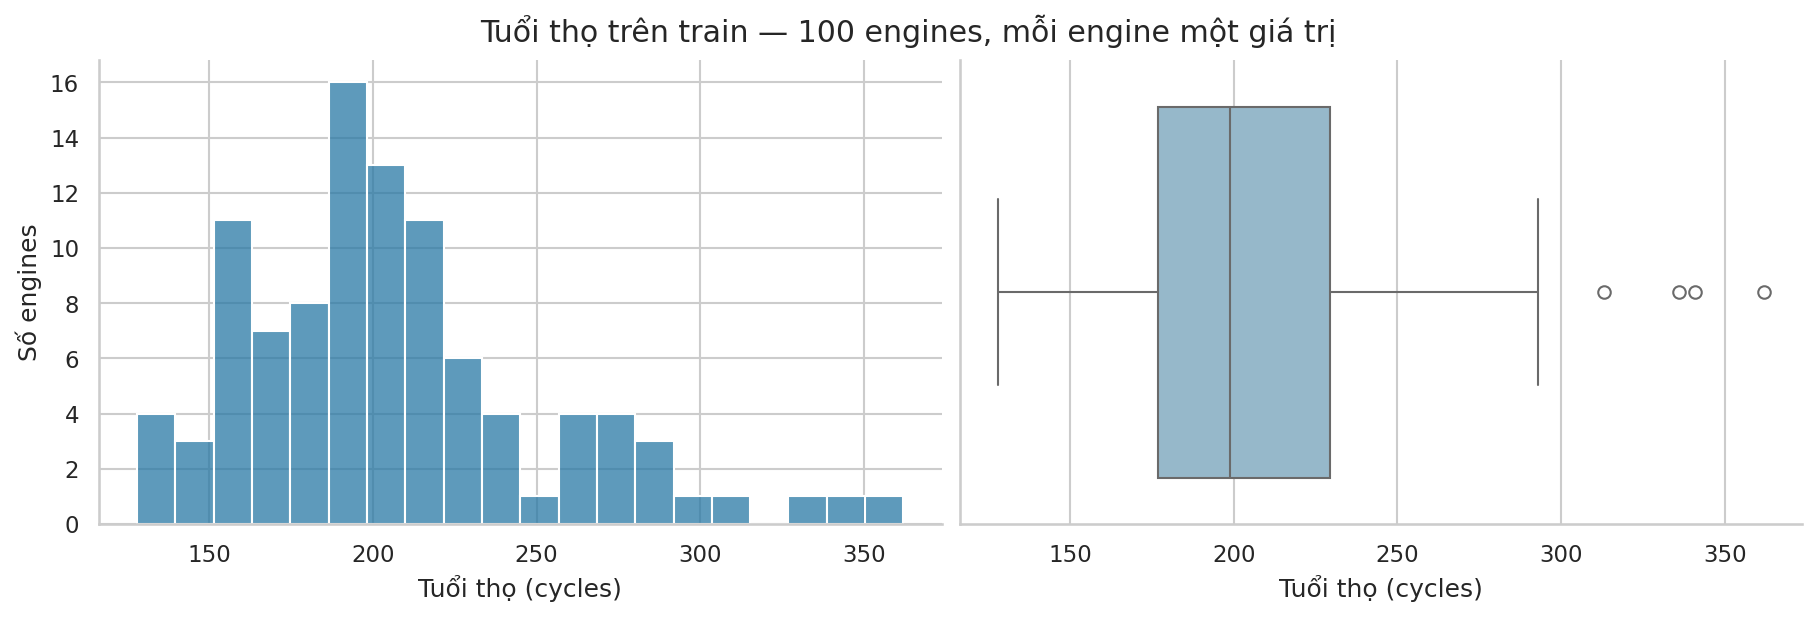
\includegraphics[width=0.9\linewidth]{../outputs/eda/figures/engine_lifetimes.png}
\caption[Phân phối tuổi thọ động cơ trên train]{Phân phối tuổi thọ train; mỗi
động cơ đóng góp một giá trị.}
\label{fig:life}
\end{figure}

Tuổi thọ dao động từ 128 đến 362 cycles; trung bình lớn hơn trung vị. Vì độ dài
chuỗi khác nhau, báo cáo phân biệt rõ tổng hợp theo observation và theo engine.
Các con số không được diễn giải thành tuổi thọ theo giờ hoặc ngày.

\subsection{Sensor hằng và correlation theo engine}
\begin{table}[H]
\centering
\caption[Correlation Spearman theo engine: các dòng minh họa]{Một số dòng minh
họa; bảng này không dùng để chọn sensor.}
\label{tab:correlation}
\begin{tabular}{lrrr}
\toprule Sensor & Động cơ xác định & Tương quan trung vị & Không xác định\\\midrule
1 & 0 & Không xác định & 100\\
6 & 62 & $-0{,}1264$ & 38\\
11 & 100 & $-0{,}8190$ & 0\\
12 & 100 & $0{,}8075$ & 0\\\bottomrule
\end{tabular}
\end{table}

Sensor 1, 5, 10, 16, 18 và 19 hằng trên train. Sensor 6 hằng trong 38/100
engine; correlation chỉ xác định trong 62 engine còn lại. Sensor 11 có tương
quan trung vị âm, còn sensor 12 có tương quan trung vị dương với RUL. Đây là
liên hệ mô tả trên train, không phải bằng chứng nhân quả hoặc hiệu quả ngoài mẫu.

\begin{figure}[H]
\centering
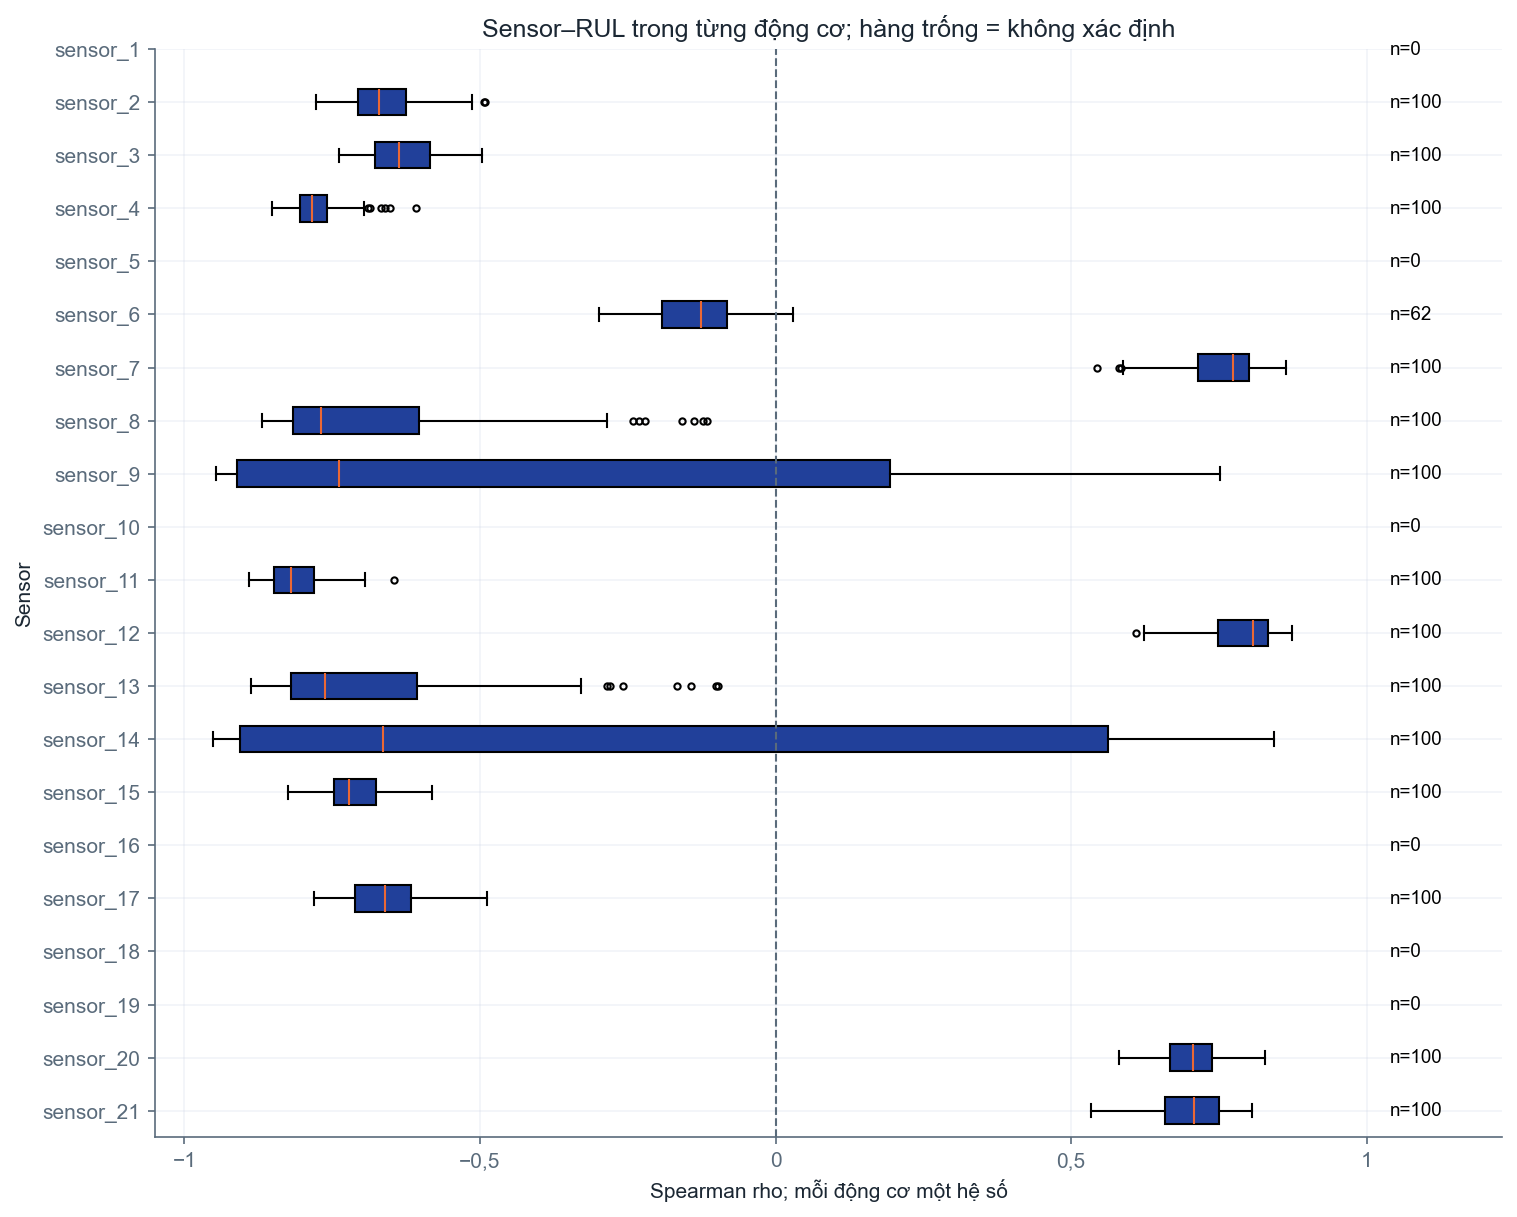
\includegraphics[width=\linewidth]{../outputs/eda/figures/sensor_rul_by_engine.png}
\caption[Phân phối correlation Spearman sensor--RUL theo động cơ]{Phân phối
correlation Spearman giữa các engine train. Sensor hằng được giữ là không xác
định.}
\label{fig:corr}
\end{figure}

\subsection{Suy luận đầu/cuối vòng đời trên train}
Bảng cặp gồm 2.100 dòng, tương ứng 100 engine train nhân 21 sensor. Mỗi dòng
dùng mean của 30 cycles đầu, mean của 30 cycles cuối và chênh lệch cuối trừ đầu.
Bảng suy luận giữ đủ 21 sensor.

Trong 21 sensor, sáu sensor có toàn bộ chênh lệch bằng 0:
\texttt{sensor\_1}, \texttt{sensor\_5}, \texttt{sensor\_10},
\texttt{sensor\_16}, \texttt{sensor\_18} và \texttt{sensor\_19}. Mười lăm
sensor còn lại kiểm định được; với cấu hình Wilcoxon permutation và
Benjamini--Hochberg trên họ 21 sensor, các p-value đã hiệu chỉnh đều xấp xỉ
0,000028.

\begin{table}[H]
\centering
\caption[Ví dụ kết quả suy luận sensor đầu/cuối]{Một số kết quả tiêu biểu. Giá
trị là chênh lệch cuối trừ đầu theo đơn vị gốc của từng sensor.}
\label{tab:sensor-inference}
\begin{tabular}{lrrl}
\toprule Sensor & Chênh lệch trung bình & Khoảng tin cậy bootstrap 95\% & Dấu chính\\\midrule
\texttt{sensor\_4} & 20,128097 & [19,402735; 20,865606] & Tăng\\
\texttt{sensor\_7} & -1,913527 & [-1,999307; -1,829684] & Giảm\\
\texttt{sensor\_11} & 0,613257 & [0,589017; 0,637944] & Tăng\\
\texttt{sensor\_12} & -1,627190 & [-1,704288; -1,552119] & Giảm\\
\texttt{sensor\_20} & -0,377007 & [-0,391534; -0,363173] & Giảm\\\bottomrule
\end{tabular}
\end{table}

\begin{figure}[H]
\centering
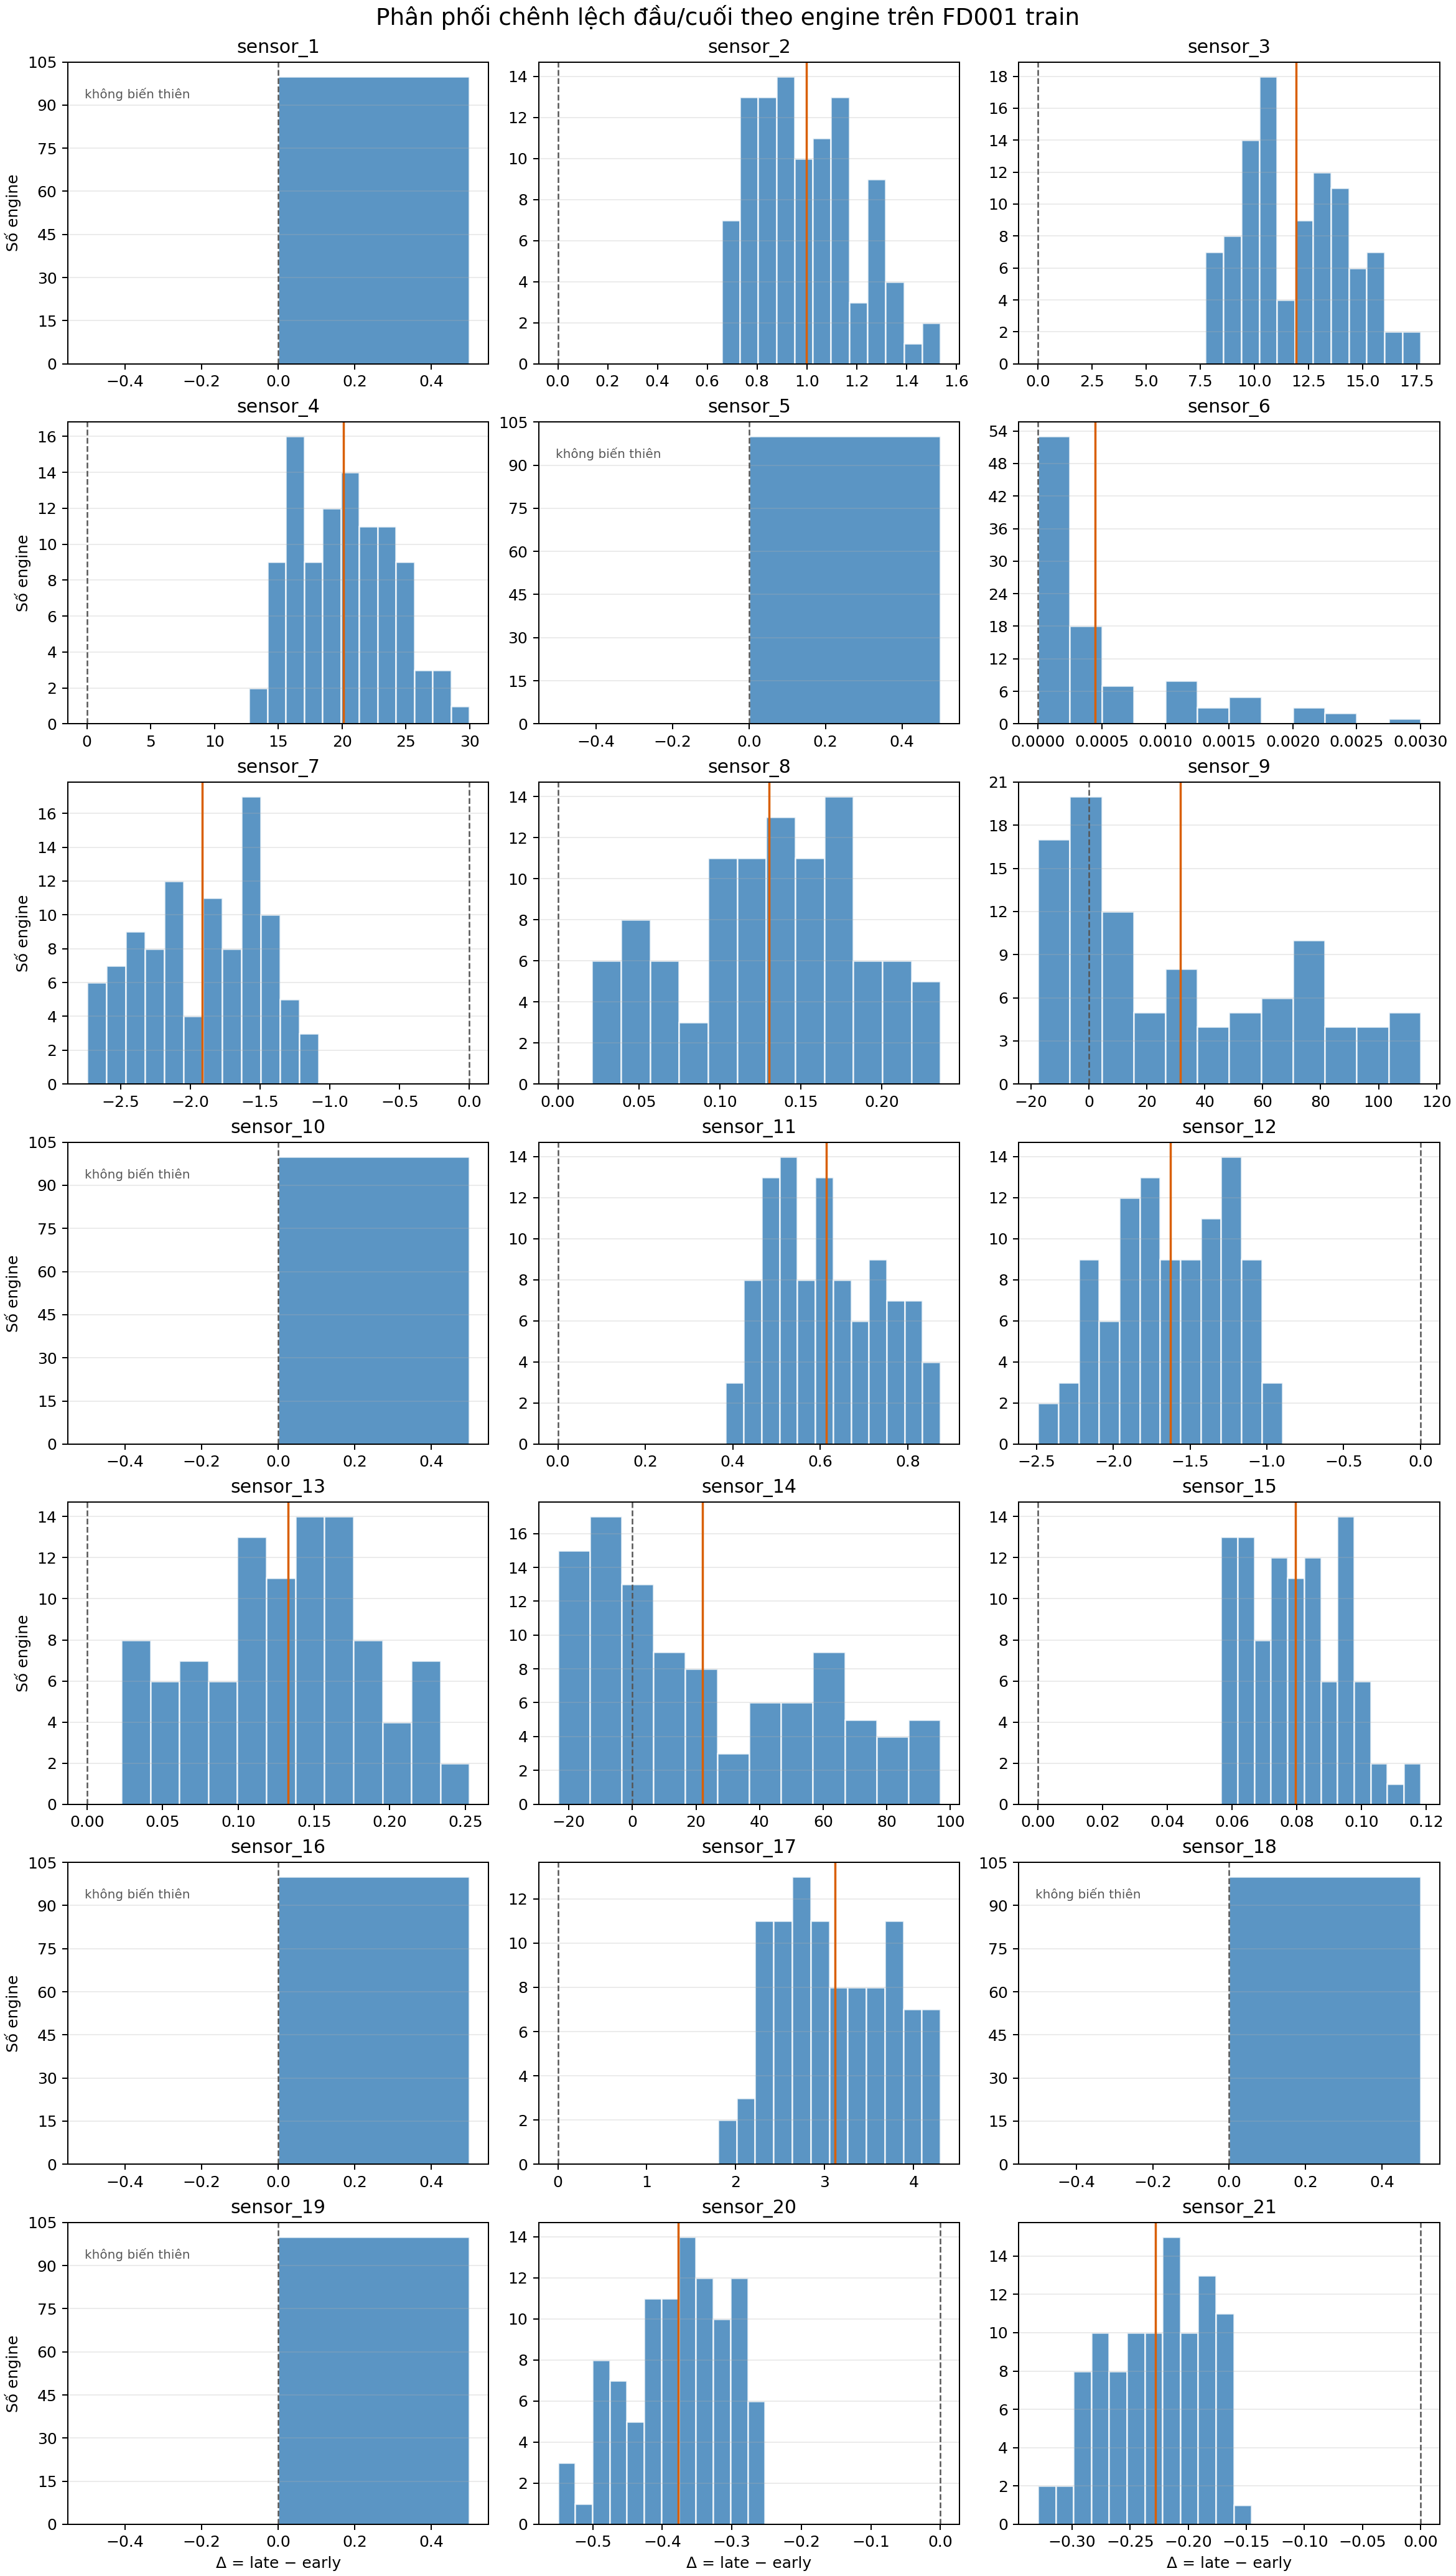
\includegraphics[width=0.86\linewidth,height=0.78\textheight,keepaspectratio]{../outputs/statistics/figures/difference_distributions.png}
\caption[Phân phối chênh lệch sensor đầu/cuối theo engine]{Phân phối chênh lệch
cuối trừ đầu của 100 engine cho từng sensor.}
\label{fig:statistics-distributions}
\end{figure}

\begin{figure}[H]
\centering
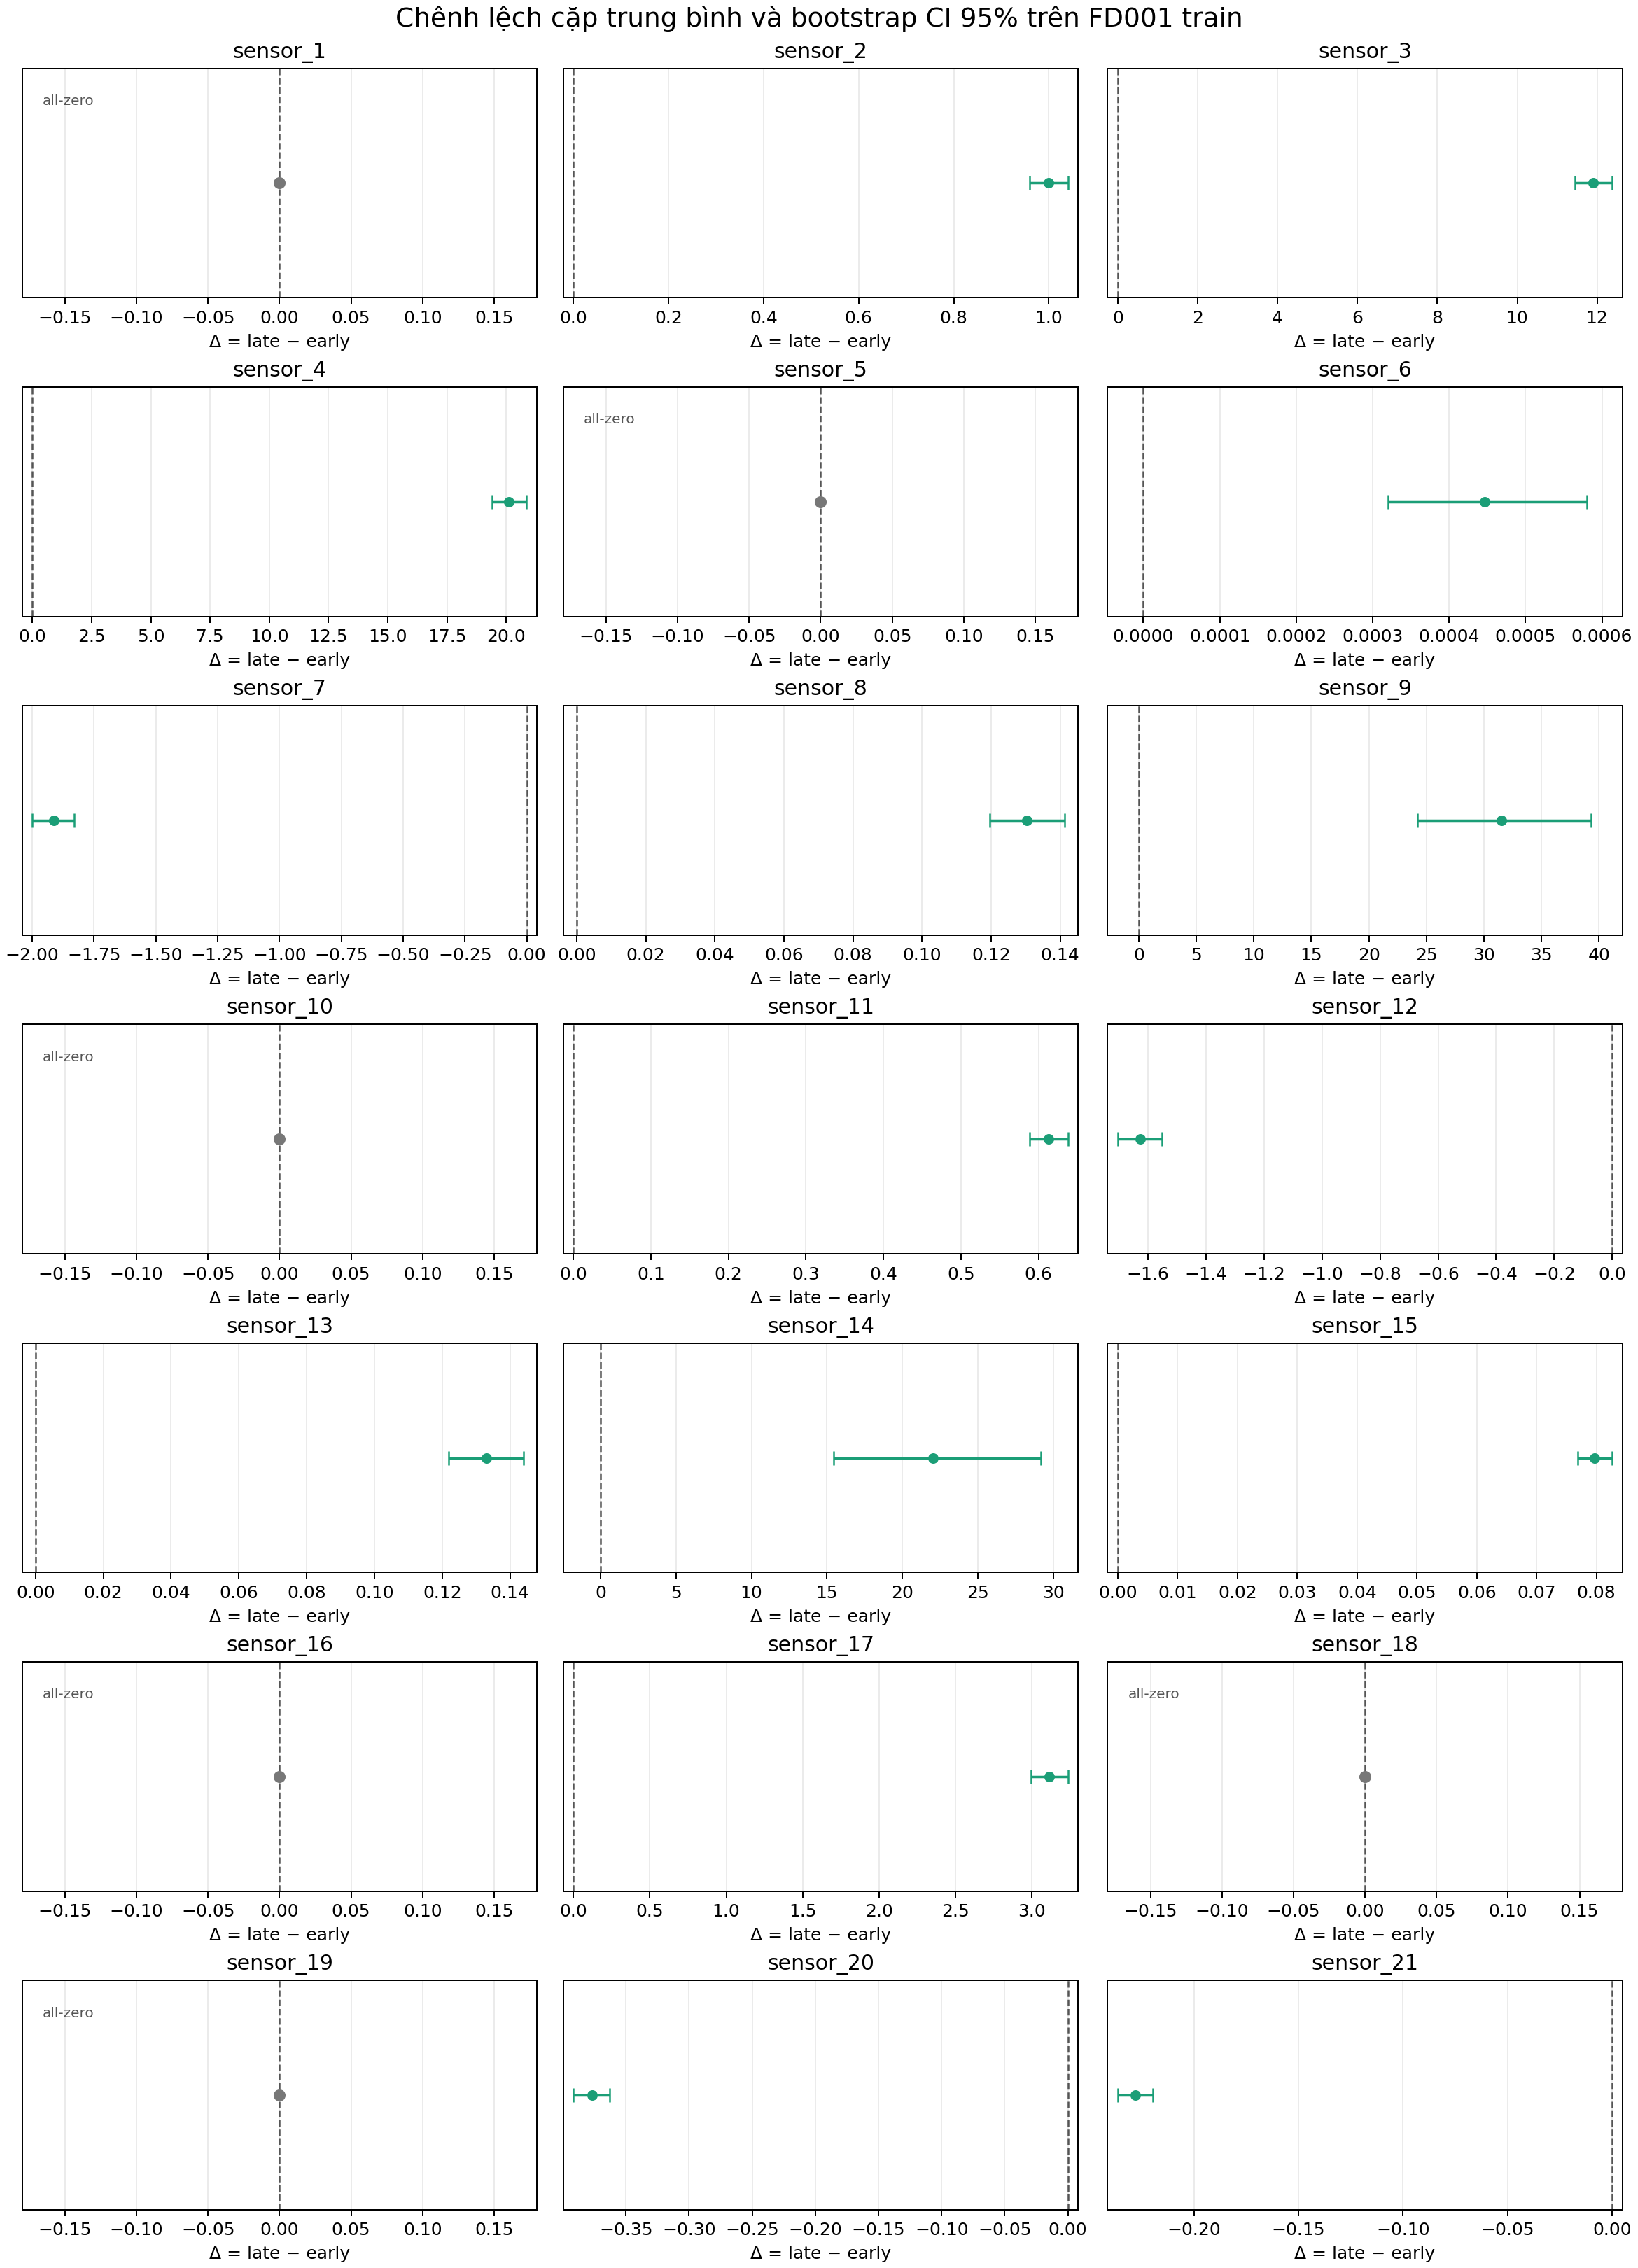
\includegraphics[width=0.86\linewidth,height=0.78\textheight,keepaspectratio]{../outputs/statistics/figures/effect_size_ci.png}
\caption[Chênh lệch cặp trung bình và khoảng tin cậy bootstrap]{Mean paired
difference và bootstrap CI 95\% theo từng sensor.}
\label{fig:statistics-effect-ci}
\end{figure}

Kết quả cho thấy nhiều sensor thay đổi có hệ thống giữa hai đoạn 30 cycles trên
train FD001 theo protocol đã chọn. Sensor 4 có chênh lệch trung bình khoảng
20,13, còn sensor 7 giảm khoảng 1,91; hai giá trị không được xếp hạng trực tiếp
vì khác thang đo. Sensor 6 có 47 chênh lệch dương và 53 chênh lệch bằng 0 nhưng
mean difference chỉ khoảng 0,00045; p-value nhỏ không đồng nghĩa thay đổi lớn.
Phân tích này không phải bằng chứng chọn feature hoặc utility dự đoán RUL ngoài
mẫu.
